\subsection{Rangefinder Implementation}
Because this device is intended to traverse unknown locations and create a 2-dimensional map, data accuracy, precision, and reliability are vital. As such, proper equipment is needed to suffice these needs. 

\subsubsection{Rangefinder Selection}
The project's rangefinder selection depended on the following criteria: field of vision, depth of sense, accuracy, precision, and cost. Many of the rangefinders limited by our budgetary restrictions were only strong in one of our project's vital criteria. However Professor Duckworth, and WPI's Electrical and Computer Engineering and Robotics Engineering Departments generously donated the URG-04LX Scanning Laser Rangefinder for the purpose of this project. The URG-04LX is a very sensitive piece of equipment that has a field of view of 240 degrees, a depth of data of 4 meters, and accuracy to within 10 millimeters, which is perfect for our application \cite{urg04lx}. Figure \ref{rangefinder_pic} below shows the rangefinder that we will be using.

\begin{figure}[H]
	\centerline{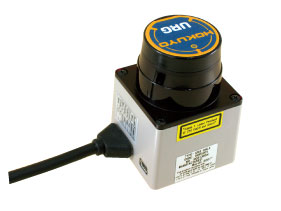
\includegraphics[width=0.5\textwidth]{urg_top.jpg}}
	\caption{URG-04LX Scanning Laser Rangefinder}
	\label{rangefinder_pic}
\end{figure}

\subsubsection{Rangefinder Communication}
The URG-04LX is very simple to use and does not require any register settings to be changed to function properly. It uses the RS-232C communication protocol, which is a form of serial differential data transmission. Thus, it recognizes a logic high from -3V to -25V and a logic low from +3V to +25V \cite{rs232}.
\par
The rangefinder can be connected to one of the ZedBoard's Pmod connectors. These Pmod connectors output data using TTL communication, which is a form of serial non-differential data transmission that recognizes a logic high of +3V to +5V and a logic low of 0V \cite{ttl}. 
\par
Since these two serial communication formats have incompatible logic levels, an RS-232 to TTL converter is needed so that the rangefinder can communicate with the ZedBoard. The converter's TTL side will be connected to the ZedBoard's Pmod connector, and the RS-232 side will be connected to the rangefinder. However, for ease of connection and testing, the 9-pin DSUB RS-232 connector will be connected to a breakout so that the pins can be easily accessed. Figure \ref{rs232_ttl_breakout} shows the RS-232 to TTL converter and the attached RS-232 breakout board.

\begin{figure}[H]
	\centerline{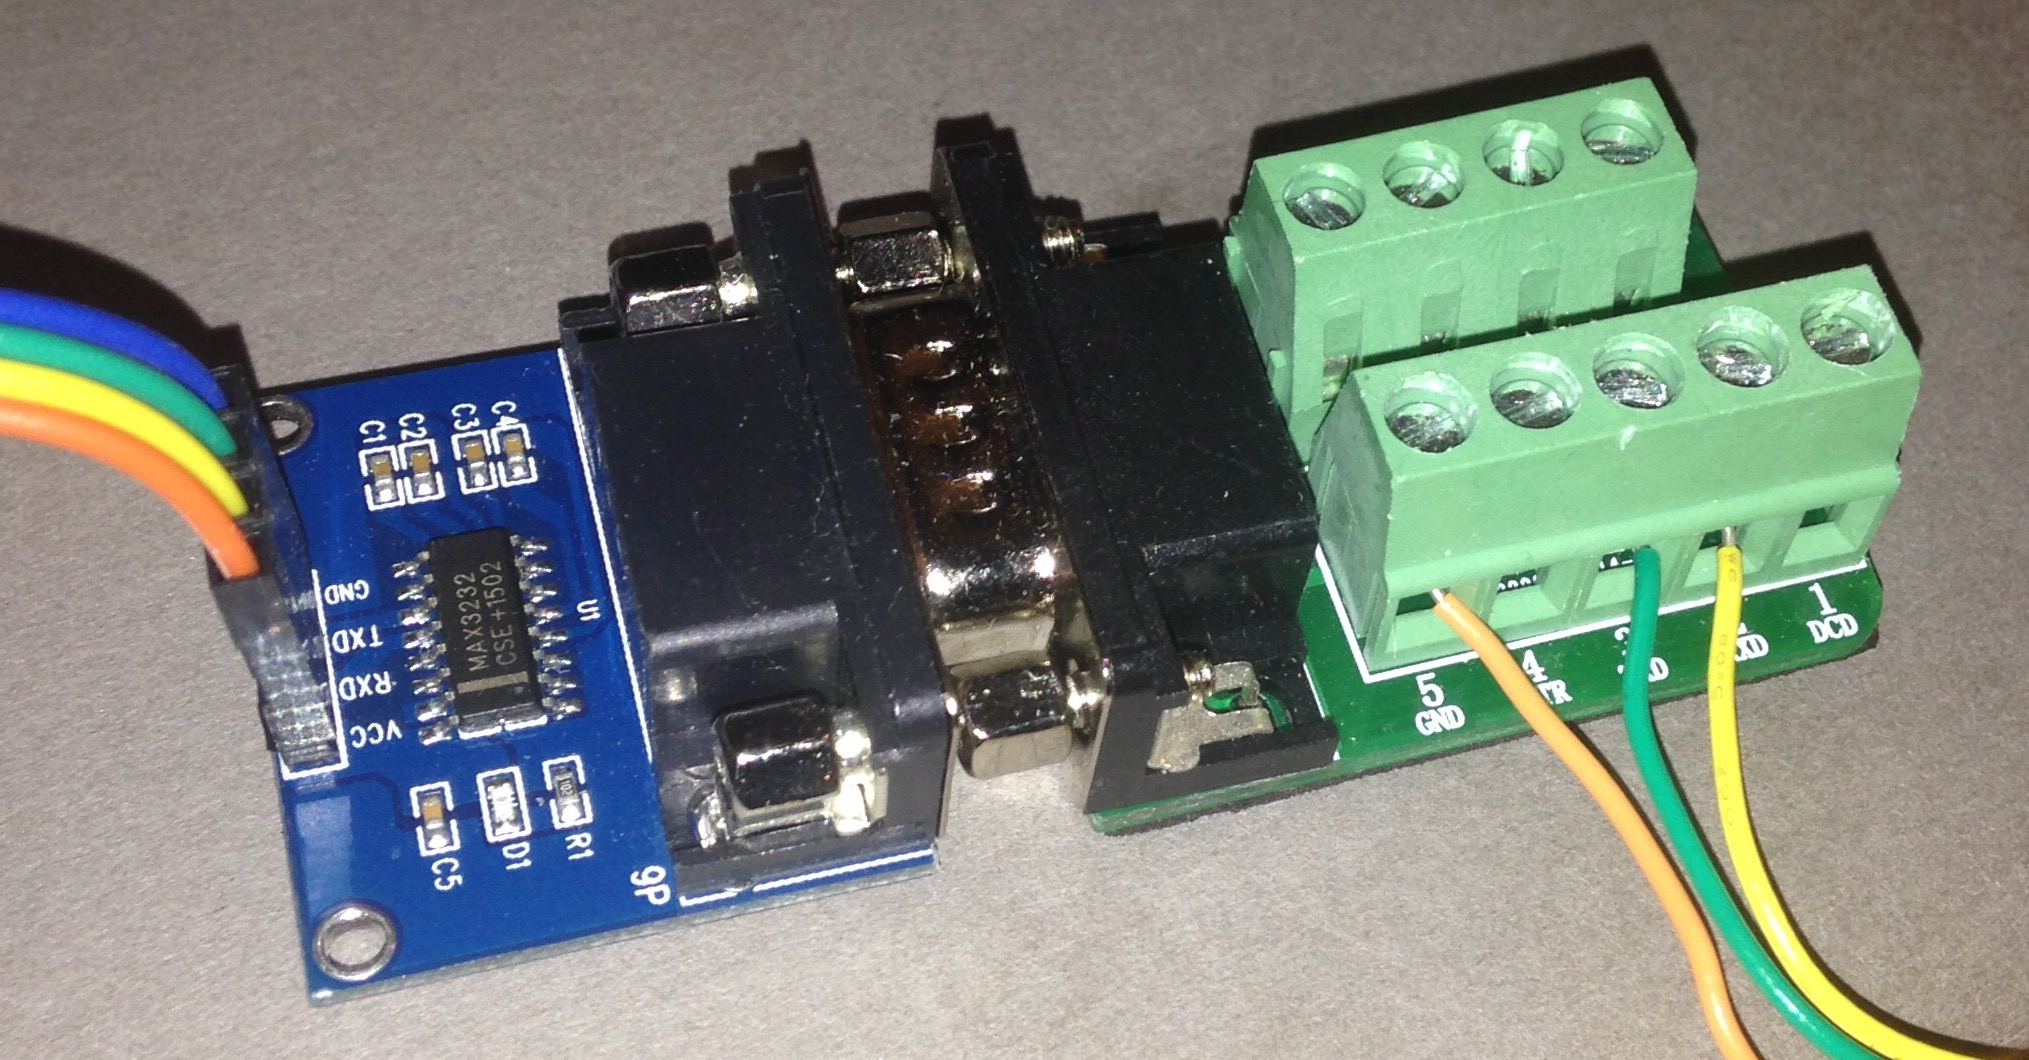
\includegraphics[width=0.5\textwidth]{rs232_ttl_breakout.png}}
	\caption{RS-232 to TTL Converter with RS-232 Breakout Board}
	\label{rs232_ttl_breakout}
\end{figure}

\subsubsection{Rangefinder Settings}